% Generated by Sphinx.
\def\sphinxdocclass{report}
\documentclass[letterpaper,10pt,french]{sphinxmanual}
\usepackage[utf8]{inputenc}
\DeclareUnicodeCharacter{00A0}{\nobreakspace}
\usepackage{cmap}
\usepackage[T1]{fontenc}
\usepackage{babel}
\usepackage{times}
\usepackage[Sonny]{fncychap}
\usepackage{longtable}
\usepackage{sphinx}
\usepackage{multirow}


\title{Documentation: dashboard professeur et développement dirigé par les tests}
\date{22 March 2015}
\release{0.1}
\author{Bryan Oberson}
\newcommand{\sphinxlogo}{}
\renewcommand{\releasename}{Version}
\makeindex

\makeatletter
\def\PYG@reset{\let\PYG@it=\relax \let\PYG@bf=\relax%
    \let\PYG@ul=\relax \let\PYG@tc=\relax%
    \let\PYG@bc=\relax \let\PYG@ff=\relax}
\def\PYG@tok#1{\csname PYG@tok@#1\endcsname}
\def\PYG@toks#1+{\ifx\relax#1\empty\else%
    \PYG@tok{#1}\expandafter\PYG@toks\fi}
\def\PYG@do#1{\PYG@bc{\PYG@tc{\PYG@ul{%
    \PYG@it{\PYG@bf{\PYG@ff{#1}}}}}}}
\def\PYG#1#2{\PYG@reset\PYG@toks#1+\relax+\PYG@do{#2}}

\expandafter\def\csname PYG@tok@gd\endcsname{\def\PYG@tc##1{\textcolor[rgb]{0.63,0.00,0.00}{##1}}}
\expandafter\def\csname PYG@tok@gu\endcsname{\let\PYG@bf=\textbf\def\PYG@tc##1{\textcolor[rgb]{0.50,0.00,0.50}{##1}}}
\expandafter\def\csname PYG@tok@gt\endcsname{\def\PYG@tc##1{\textcolor[rgb]{0.00,0.27,0.87}{##1}}}
\expandafter\def\csname PYG@tok@gs\endcsname{\let\PYG@bf=\textbf}
\expandafter\def\csname PYG@tok@gr\endcsname{\def\PYG@tc##1{\textcolor[rgb]{1.00,0.00,0.00}{##1}}}
\expandafter\def\csname PYG@tok@cm\endcsname{\let\PYG@it=\textit\def\PYG@tc##1{\textcolor[rgb]{0.25,0.50,0.56}{##1}}}
\expandafter\def\csname PYG@tok@vg\endcsname{\def\PYG@tc##1{\textcolor[rgb]{0.73,0.38,0.84}{##1}}}
\expandafter\def\csname PYG@tok@m\endcsname{\def\PYG@tc##1{\textcolor[rgb]{0.13,0.50,0.31}{##1}}}
\expandafter\def\csname PYG@tok@mh\endcsname{\def\PYG@tc##1{\textcolor[rgb]{0.13,0.50,0.31}{##1}}}
\expandafter\def\csname PYG@tok@cs\endcsname{\def\PYG@tc##1{\textcolor[rgb]{0.25,0.50,0.56}{##1}}\def\PYG@bc##1{\setlength{\fboxsep}{0pt}\colorbox[rgb]{1.00,0.94,0.94}{\strut ##1}}}
\expandafter\def\csname PYG@tok@ge\endcsname{\let\PYG@it=\textit}
\expandafter\def\csname PYG@tok@vc\endcsname{\def\PYG@tc##1{\textcolor[rgb]{0.73,0.38,0.84}{##1}}}
\expandafter\def\csname PYG@tok@il\endcsname{\def\PYG@tc##1{\textcolor[rgb]{0.13,0.50,0.31}{##1}}}
\expandafter\def\csname PYG@tok@go\endcsname{\def\PYG@tc##1{\textcolor[rgb]{0.20,0.20,0.20}{##1}}}
\expandafter\def\csname PYG@tok@cp\endcsname{\def\PYG@tc##1{\textcolor[rgb]{0.00,0.44,0.13}{##1}}}
\expandafter\def\csname PYG@tok@gi\endcsname{\def\PYG@tc##1{\textcolor[rgb]{0.00,0.63,0.00}{##1}}}
\expandafter\def\csname PYG@tok@gh\endcsname{\let\PYG@bf=\textbf\def\PYG@tc##1{\textcolor[rgb]{0.00,0.00,0.50}{##1}}}
\expandafter\def\csname PYG@tok@ni\endcsname{\let\PYG@bf=\textbf\def\PYG@tc##1{\textcolor[rgb]{0.84,0.33,0.22}{##1}}}
\expandafter\def\csname PYG@tok@nl\endcsname{\let\PYG@bf=\textbf\def\PYG@tc##1{\textcolor[rgb]{0.00,0.13,0.44}{##1}}}
\expandafter\def\csname PYG@tok@nn\endcsname{\let\PYG@bf=\textbf\def\PYG@tc##1{\textcolor[rgb]{0.05,0.52,0.71}{##1}}}
\expandafter\def\csname PYG@tok@no\endcsname{\def\PYG@tc##1{\textcolor[rgb]{0.38,0.68,0.84}{##1}}}
\expandafter\def\csname PYG@tok@na\endcsname{\def\PYG@tc##1{\textcolor[rgb]{0.25,0.44,0.63}{##1}}}
\expandafter\def\csname PYG@tok@nb\endcsname{\def\PYG@tc##1{\textcolor[rgb]{0.00,0.44,0.13}{##1}}}
\expandafter\def\csname PYG@tok@nc\endcsname{\let\PYG@bf=\textbf\def\PYG@tc##1{\textcolor[rgb]{0.05,0.52,0.71}{##1}}}
\expandafter\def\csname PYG@tok@nd\endcsname{\let\PYG@bf=\textbf\def\PYG@tc##1{\textcolor[rgb]{0.33,0.33,0.33}{##1}}}
\expandafter\def\csname PYG@tok@ne\endcsname{\def\PYG@tc##1{\textcolor[rgb]{0.00,0.44,0.13}{##1}}}
\expandafter\def\csname PYG@tok@nf\endcsname{\def\PYG@tc##1{\textcolor[rgb]{0.02,0.16,0.49}{##1}}}
\expandafter\def\csname PYG@tok@si\endcsname{\let\PYG@it=\textit\def\PYG@tc##1{\textcolor[rgb]{0.44,0.63,0.82}{##1}}}
\expandafter\def\csname PYG@tok@s2\endcsname{\def\PYG@tc##1{\textcolor[rgb]{0.25,0.44,0.63}{##1}}}
\expandafter\def\csname PYG@tok@vi\endcsname{\def\PYG@tc##1{\textcolor[rgb]{0.73,0.38,0.84}{##1}}}
\expandafter\def\csname PYG@tok@nt\endcsname{\let\PYG@bf=\textbf\def\PYG@tc##1{\textcolor[rgb]{0.02,0.16,0.45}{##1}}}
\expandafter\def\csname PYG@tok@nv\endcsname{\def\PYG@tc##1{\textcolor[rgb]{0.73,0.38,0.84}{##1}}}
\expandafter\def\csname PYG@tok@s1\endcsname{\def\PYG@tc##1{\textcolor[rgb]{0.25,0.44,0.63}{##1}}}
\expandafter\def\csname PYG@tok@gp\endcsname{\let\PYG@bf=\textbf\def\PYG@tc##1{\textcolor[rgb]{0.78,0.36,0.04}{##1}}}
\expandafter\def\csname PYG@tok@sh\endcsname{\def\PYG@tc##1{\textcolor[rgb]{0.25,0.44,0.63}{##1}}}
\expandafter\def\csname PYG@tok@ow\endcsname{\let\PYG@bf=\textbf\def\PYG@tc##1{\textcolor[rgb]{0.00,0.44,0.13}{##1}}}
\expandafter\def\csname PYG@tok@sx\endcsname{\def\PYG@tc##1{\textcolor[rgb]{0.78,0.36,0.04}{##1}}}
\expandafter\def\csname PYG@tok@bp\endcsname{\def\PYG@tc##1{\textcolor[rgb]{0.00,0.44,0.13}{##1}}}
\expandafter\def\csname PYG@tok@c1\endcsname{\let\PYG@it=\textit\def\PYG@tc##1{\textcolor[rgb]{0.25,0.50,0.56}{##1}}}
\expandafter\def\csname PYG@tok@kc\endcsname{\let\PYG@bf=\textbf\def\PYG@tc##1{\textcolor[rgb]{0.00,0.44,0.13}{##1}}}
\expandafter\def\csname PYG@tok@c\endcsname{\let\PYG@it=\textit\def\PYG@tc##1{\textcolor[rgb]{0.25,0.50,0.56}{##1}}}
\expandafter\def\csname PYG@tok@mf\endcsname{\def\PYG@tc##1{\textcolor[rgb]{0.13,0.50,0.31}{##1}}}
\expandafter\def\csname PYG@tok@err\endcsname{\def\PYG@bc##1{\setlength{\fboxsep}{0pt}\fcolorbox[rgb]{1.00,0.00,0.00}{1,1,1}{\strut ##1}}}
\expandafter\def\csname PYG@tok@kd\endcsname{\let\PYG@bf=\textbf\def\PYG@tc##1{\textcolor[rgb]{0.00,0.44,0.13}{##1}}}
\expandafter\def\csname PYG@tok@ss\endcsname{\def\PYG@tc##1{\textcolor[rgb]{0.32,0.47,0.09}{##1}}}
\expandafter\def\csname PYG@tok@sr\endcsname{\def\PYG@tc##1{\textcolor[rgb]{0.14,0.33,0.53}{##1}}}
\expandafter\def\csname PYG@tok@mo\endcsname{\def\PYG@tc##1{\textcolor[rgb]{0.13,0.50,0.31}{##1}}}
\expandafter\def\csname PYG@tok@mi\endcsname{\def\PYG@tc##1{\textcolor[rgb]{0.13,0.50,0.31}{##1}}}
\expandafter\def\csname PYG@tok@kn\endcsname{\let\PYG@bf=\textbf\def\PYG@tc##1{\textcolor[rgb]{0.00,0.44,0.13}{##1}}}
\expandafter\def\csname PYG@tok@o\endcsname{\def\PYG@tc##1{\textcolor[rgb]{0.40,0.40,0.40}{##1}}}
\expandafter\def\csname PYG@tok@kr\endcsname{\let\PYG@bf=\textbf\def\PYG@tc##1{\textcolor[rgb]{0.00,0.44,0.13}{##1}}}
\expandafter\def\csname PYG@tok@s\endcsname{\def\PYG@tc##1{\textcolor[rgb]{0.25,0.44,0.63}{##1}}}
\expandafter\def\csname PYG@tok@kp\endcsname{\def\PYG@tc##1{\textcolor[rgb]{0.00,0.44,0.13}{##1}}}
\expandafter\def\csname PYG@tok@w\endcsname{\def\PYG@tc##1{\textcolor[rgb]{0.73,0.73,0.73}{##1}}}
\expandafter\def\csname PYG@tok@kt\endcsname{\def\PYG@tc##1{\textcolor[rgb]{0.56,0.13,0.00}{##1}}}
\expandafter\def\csname PYG@tok@sc\endcsname{\def\PYG@tc##1{\textcolor[rgb]{0.25,0.44,0.63}{##1}}}
\expandafter\def\csname PYG@tok@sb\endcsname{\def\PYG@tc##1{\textcolor[rgb]{0.25,0.44,0.63}{##1}}}
\expandafter\def\csname PYG@tok@k\endcsname{\let\PYG@bf=\textbf\def\PYG@tc##1{\textcolor[rgb]{0.00,0.44,0.13}{##1}}}
\expandafter\def\csname PYG@tok@se\endcsname{\let\PYG@bf=\textbf\def\PYG@tc##1{\textcolor[rgb]{0.25,0.44,0.63}{##1}}}
\expandafter\def\csname PYG@tok@sd\endcsname{\let\PYG@it=\textit\def\PYG@tc##1{\textcolor[rgb]{0.25,0.44,0.63}{##1}}}

\def\PYGZbs{\char`\\}
\def\PYGZus{\char`\_}
\def\PYGZob{\char`\{}
\def\PYGZcb{\char`\}}
\def\PYGZca{\char`\^}
\def\PYGZam{\char`\&}
\def\PYGZlt{\char`\<}
\def\PYGZgt{\char`\>}
\def\PYGZsh{\char`\#}
\def\PYGZpc{\char`\%}
\def\PYGZdl{\char`\$}
\def\PYGZhy{\char`\-}
\def\PYGZsq{\char`\'}
\def\PYGZdq{\char`\"}
\def\PYGZti{\char`\~}
% for compatibility with earlier versions
\def\PYGZat{@}
\def\PYGZlb{[}
\def\PYGZrb{]}
\makeatother

\renewcommand\PYGZsq{\textquotesingle}

\begin{document}

\maketitle
\tableofcontents
\phantomsection\label{index::doc}



\chapter{Introduction}
\label{introduction:introduction}\label{introduction:conception-du-dashboard-professeur-a-laide-du-developpement-dirige-par-les-tests}\label{introduction::doc}
Dans ce travail, je vais tout d'abord documenter mon travail pratique. Ce
travail consiste en la conception d'un dashboard pour les professeurs
utilisant le framework Django tout en essayant de programmer
avec le développement dirigé par les tests.
Ce dashboard fera partie d'un projet plus grand: un site d'e-learning pour les
mathématiques.
Tous les termes spécifiques tels que framework seront expliqués par la suite.

Cette documentation parlera tout d'abord de l'intérêt de ce travail pratique.
Il y aura aussi le wireframe du dashboard et un diagramme UML expliquant mes
différents modèles Django. J'expliquerai par la suite comment j'ai utilisé
les différentes technologies pour créer mon application et comment
je pourrai l'intégrer au projet final (le site) en essayant de souligner les
difficultés que je pourrai rencontrer pendant l'intégration.

Par la suite, j'essaierai de résumer les connaissances de bases relatives
au développement dirigé par les tests. Ceci consistera à expliquer les
différents termes et à surtout à expliquer comment cela fonctionne et quels
sont les avantages.

Finalement, j'expliquerai comment créer une ébauche de dashboard (créer un
dashboard complet étant trop long et trop compliqué à tester de par le nombre
important de boutons et de fonctionnalités) en utilisant ce fameux
développement dirigé par les tests


\chapter{Explications des termes spécifiques}
\label{introduction:explications-des-termes-specifiques}
Pour être sûr que tout le monde comprenne de quoi nous allons parler,
il va nous falloir expliquer le lexique spécifique à nos deux sujets:
dashboard professeur et développement dirigé par les tests.


\section{Framework}
\label{introduction:framework}
Un \textbf{framework}, ou \textbf{structure logicielle}, sert de base à un programme.
En effet, c'est de par ses structures de base que l'on peut le plus facilement
programmer. C'est donc une grande aide à tout informaticien. Les framework les
plus connus seraient, par exemple, Django, Bootstrap ou Ruby On Rails.

Il est important de noter que les frameworks sont souvent spécialisés dans un
langage informatique très précis. Par exemple, Django utilise Python, Bootstrap
utilise HTML et CSS et Ruby on Rails utilise Ruby.

Un framework est en autre très utile pour la programmation orientée objet. Ce
type de programmation permet d'établir des liens entre les différents objets.
Le framework aide à créer des classes et surtout des héritages.


\section{Classes et héritages}
\label{introduction:classes-et-heritages}
Les \textbf{classes} correspondent à un moule dans lequel on met différentes
informations pour créer un objet. Par exemple, pour une voiture, on pourrait
définir sa couleur, sa marque ou encore son age. Tout ce qu'il reste à faire
est de donner des valeurs à ces trois propriétés pour ``créer'' la voiture.

Le concept d'héritage n'est pas beaucoup plus compliqué. En effet, un héritage
consiste à créer une classe en prenant comme base les caractéristiques d'une
autre, ce qui nous permet d'en rajouter d'autre. Dans un cas qui nous
intéresserait plus, un élève possède comme spécificités un nom, un prénom et
une école. On peut grâce à ça créer une classe Professeur, qui aura les
mêmes caractéristiques mais à laquelle on pourrait ajouter la branche qu'il
enseigne.


\section{Diagramme UML}
\label{introduction:diagramme-uml}
Quand l'on possède de nombreuses classes, il devient indispensable de pouvoir
voir rapidement quelles relations ces classes entreprennent entre elles. Pour
ceci, le meilleur moyen de le faire est de créer un \textbf{diagramme UML}. Un diagramme
schématise les objets et indique leurs différentes relations (relation simple
avec une clé étrangère ou aussi plusieurs-à-plusieurs (ManyToMany)).

Il existe de nombreux programmes permettant de réaliser des diagrammes UML
clairs et présentables, comme boUML, argoUML ou Poseidon.


\section{Wireframe}
\label{introduction:wireframe}
Un \textbf{wireframe} est un schéma consistant à mettre en valeur les relations entre les
différentes pages d'un site web. Cela explique par exemple ce qu'il se passe si
l'on clique sur tel ou tel bouton. Cela consiste donc à pouvoir voir ou
exactement l'on peut aller en manipulant les fonctionnalités du site.


\chapter{Fonctionnalités du dashboard}
\label{dashboard:fonctionnalites-du-dashboard}\label{dashboard::doc}

\section{Ajouter un groupe}
\label{dashboard:ajouter-un-groupe}
La fonctionnalité de base de ce dashboard est la création de groupe. En créant
un groupe, le professeur sera par la suite capable de le gérer en gérant les
membres qui s'y trouvent mais aussi en y assignant des devoirs.

Pour créer un groupe, il suffit de se rendre sur Nouveau groupe, tout en bas
dans le menu de gauche. Cette action fera apparaître le formulaire de création
de groupe.
\begin{figure}[htbp]
\centering
\capstart

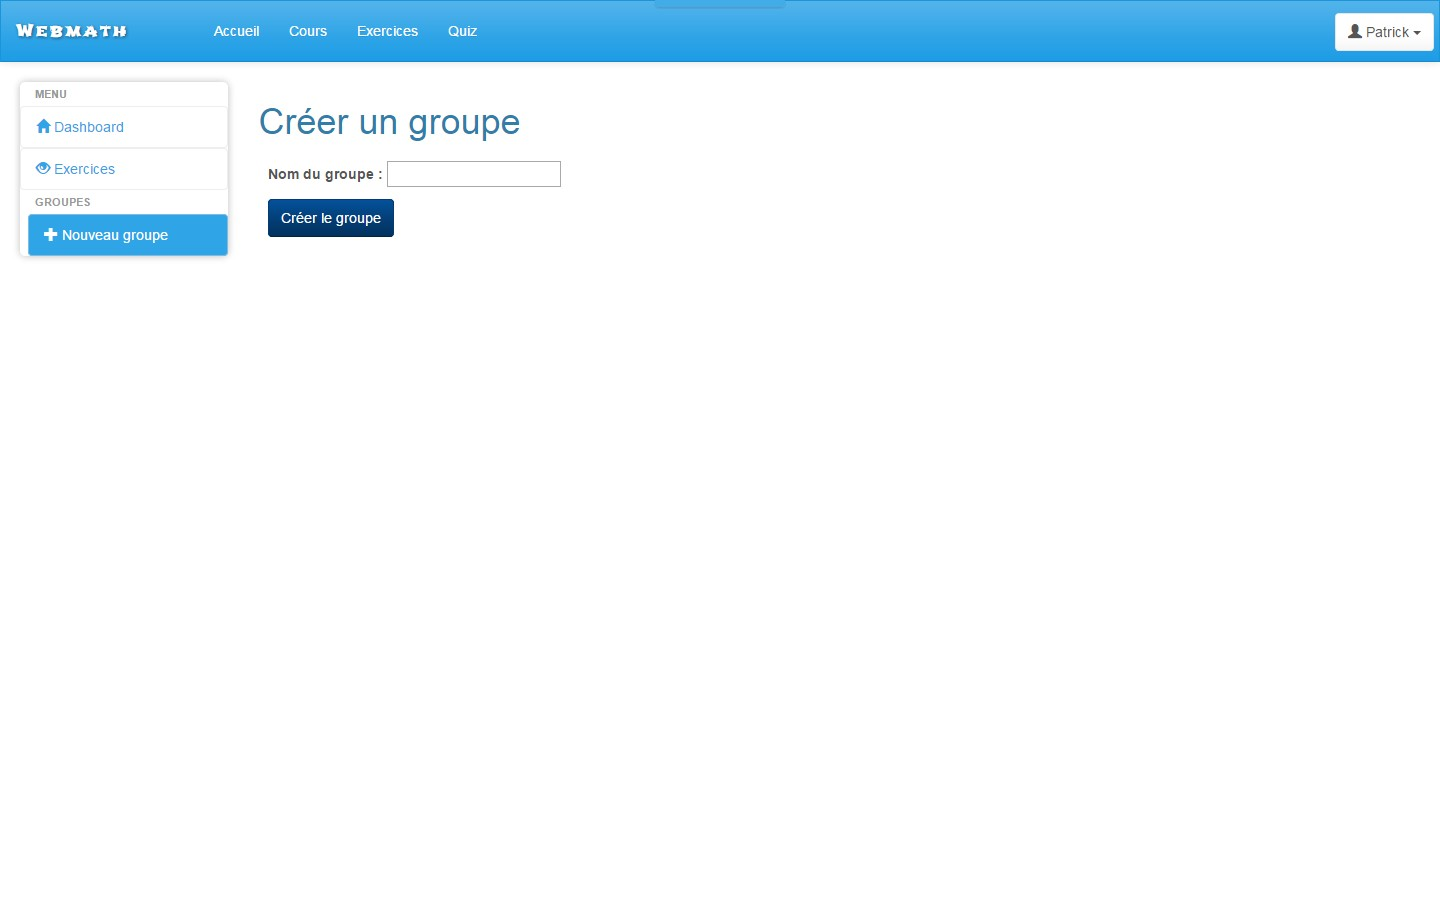
\includegraphics[width=0.700\linewidth]{Newclass.jpg}
\caption{Formulaire de création de groupe}\end{figure}

La seule exigence présente lors de la création d'un groupe est le nom. Une fois
le groupe créé, l'utilisateur actuel est automatiquement défini en tant que
professeur pour le groupe.

Le groupe précédemment créé sera désormais affiché en permanence dans le menu
de gauche du professeur, ce qui lui permet d'accéder à ses informations.


\section{Gérer un groupe}
\label{dashboard:gerer-un-groupe}

\subsection{Gérer les membres du groupe}
\label{dashboard:gerer-les-membres-du-groupe}
Depuis cette page, le professeur peut gérer les membres qui sont actuellement
enregistrés dans le groupe.

Il peut tout d'abord rajouter les élèves ou professeurs qu'il souhaite en
entrant leur nom d'utilisateur dans le champ à disposition.
\begin{figure}[htbp]
\centering
\capstart

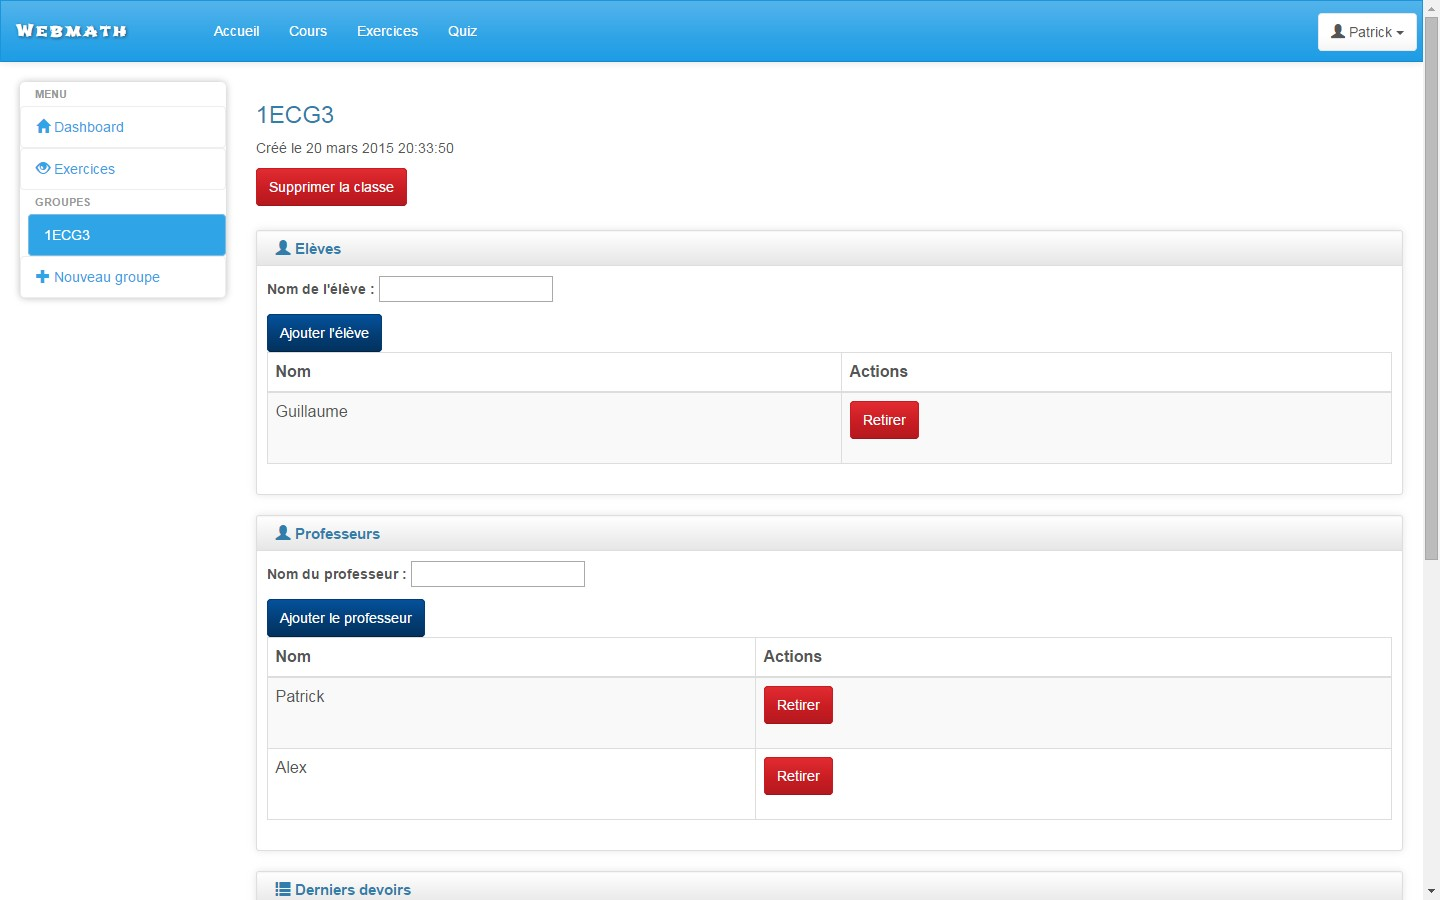
\includegraphics[width=0.700\linewidth]{class.jpg}
\caption{Page d'administration d'un groupe}\end{figure}

Si le nom d'utilisateur rentré correspond bien à un étudiant ou à un professeur,
cet utilisateur sera rajouté dans la liste des membres.
\begin{figure}[htbp]
\centering
\capstart

\includegraphics[width=0.700\linewidth]{classAjouterMembres.jpg}
\caption{Ce à quoi ressemble la page une fois que des membres ont été rajoutés}\end{figure}

Au contraire, si aucun utilisateur n'a été trouvé ou si l'utilisateur ne
correspond pas au rôle qu'il lui est donné (par exemple si c'est un
professeur et qu'il a été ajouté aux étudiants), le site renvoiera un message
d'erreur.
\begin{figure}[htbp]
\centering
\capstart

\includegraphics[width=0.700\linewidth]{classAjouterMembresEchec.jpg}
\caption{Message d'erreur retourné si l'utilisateur n'est pas valable}\end{figure}

Une fois ajouté, un membre peut facilement être retiré du groupe grâce au bouton
Retirer qui se trouve à côté de son nom.


\subsection{Gérer un devoir}
\label{dashboard:gerer-un-devoir}
Un professeur peut bien évidemment donner des devoirs à son groupe.

Un devoir peut-être un exercice, un quiz ou un cours, tous les trois
pouvant avoir été créé par un autre utilisateur.

Pour assigner un devoir, il suffit de savoir l'id de l'exercice, quiz ou cours,
et de préciser grâce au menu à choix de quel type de devoir il s'agit.
\begin{figure}[htbp]
\centering
\capstart

\includegraphics[width=0.700\linewidth]{classDevoir.jpg}
\caption{Différents champs à compléter pour assigner un devoir}\end{figure}

Comme pour les fonctionnalités précédentes, si aucun exercice, quiz ou cours
n'a pu être associé à l'id entrée, un message d'erreur sera renvoyé.

Un devoir peut être à tout moment retiré grâce au bouton Retirer à sa droite.


\section{Voir ses exercices}
\label{dashboard:voir-ses-exercices}
Dans le menu de gauche, il y a un bouton nommé Exercices. C'est depuis cette
page que le professeur pourra voir ses exercices, ses quiz et ses cours.
\begin{figure}[htbp]
\centering
\capstart

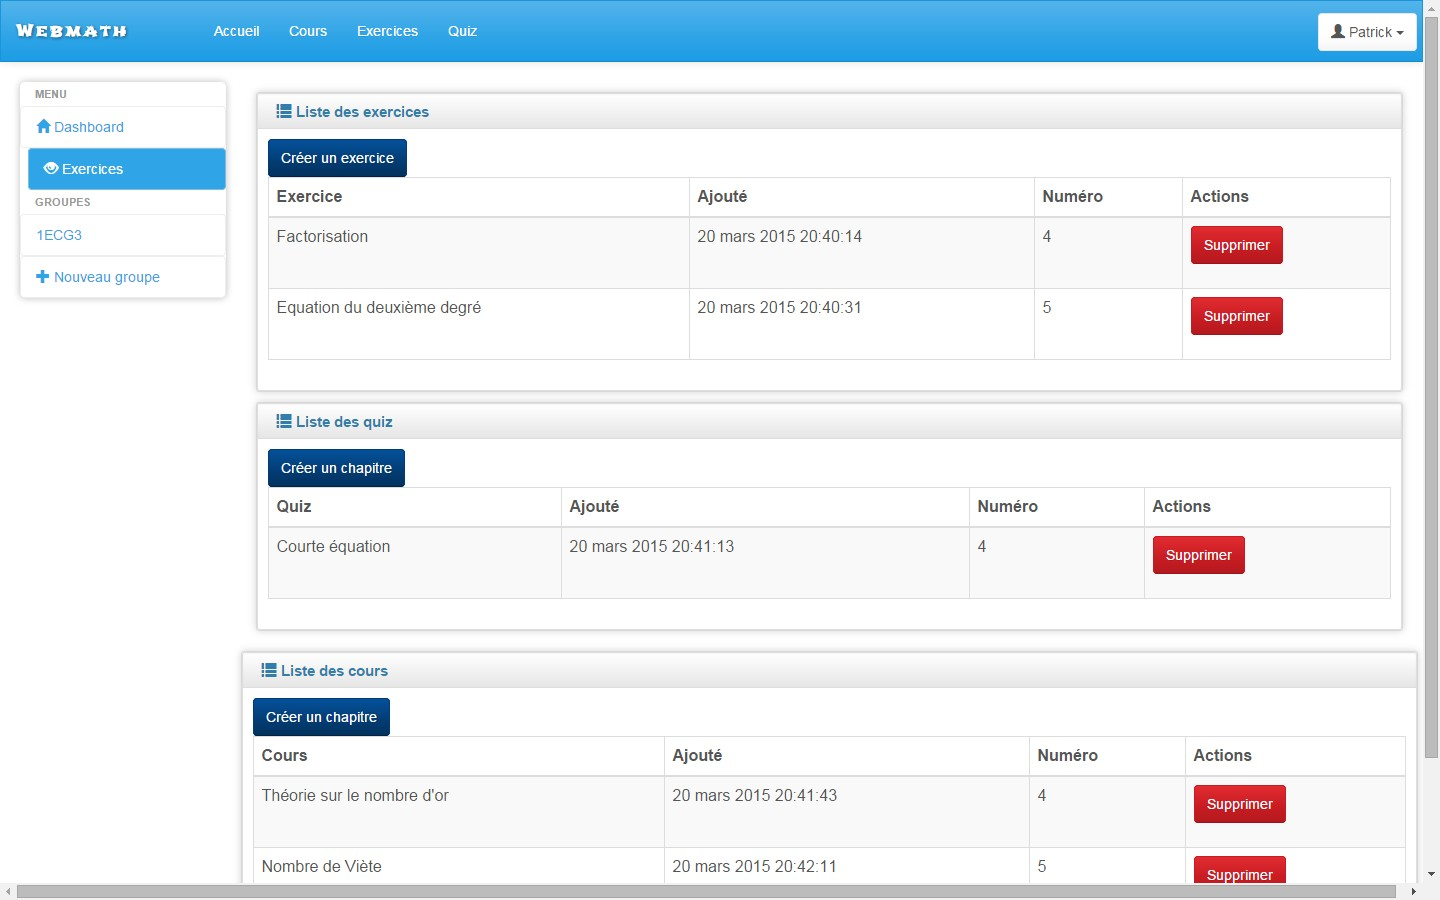
\includegraphics[width=0.700\linewidth]{exercices.jpg}
\caption{Ce à quoi ressemble la page Exercices}\end{figure}

Pour chaque activité que le professeur aura créé, il pourra voir le titre qu'il
lui a donné, la date à laquelle il l'a créé et l'id qui lui sera utile s'il veut
l'assigner en tant que devoir à un de ses groupes.

Il peut bien évidemment supprimer une activité en utilisant le bouton Supprimer
se trouvant dans la dernière colonne du tableau.

Si le professeur souhaite créer une nouvelle activité, il n'a qu'à utiliser le
bouton Créer en haut du tableau qui le redirigera directement au formulaire de
création.


\section{Changer de mot de passe}
\label{dashboard:changer-de-mot-de-passe}
Peu importe sur quelle page il se trouve, le professeur peut accéder à un menu
déroulant en haut à droite de cette page.
\begin{figure}[htbp]
\centering
\capstart

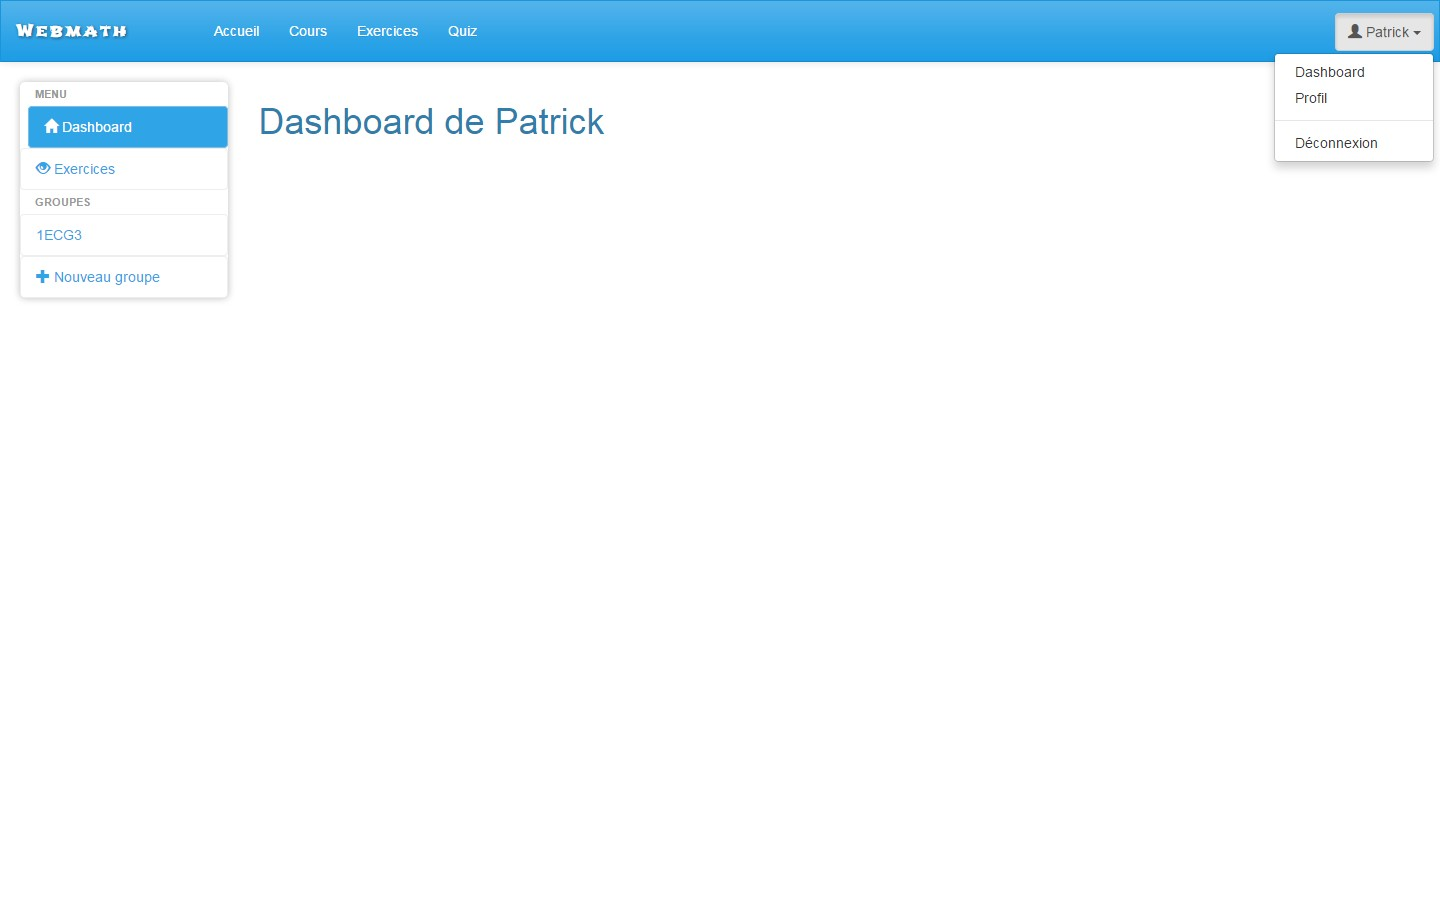
\includegraphics[width=0.700\linewidth]{menuDeroulant.jpg}
\caption{Apparence du menu déroulant}\end{figure}

Dashboard amène le professeur sur l'accueil de son dashboard, Déconnexion le
déconnecte et Profil l'amène sur un formulaire de changement de mot de passe.

Pour le modifier, le professeur n'a qu'à remplir les deux champs et à valider.
Si tout a été rentré correctement, le mot de passe sera correctement modifié.
\begin{figure}[htbp]
\centering
\capstart

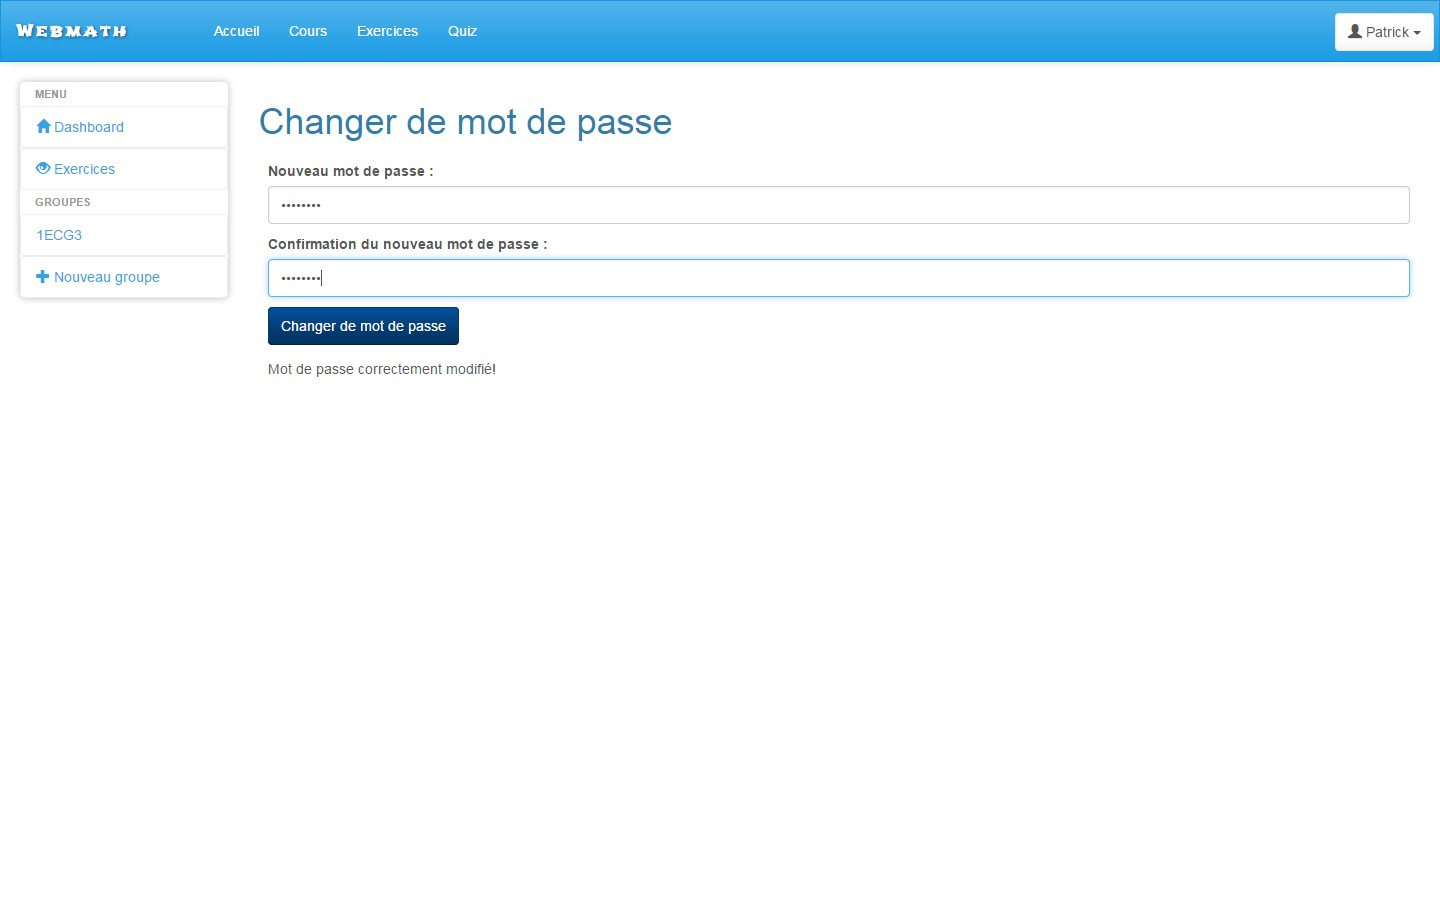
\includegraphics[width=0.700\linewidth]{passwordSuccess.jpg}
\caption{Message pour confirmer que le changement de mot de passe a correctement eu
lieu}\end{figure}

Au contraire, s'il y a une erreur, un message d'erreur sera retourné.
\begin{figure}[htbp]
\centering
\capstart

\includegraphics[width=0.700\linewidth]{passwordFail.jpg}
\caption{Message d'erreur retourné si les champs n'ont pas correctement été remplis}\end{figure}


\chapter{Documentation}
\label{documentation:documentation}\label{documentation::doc}

\section{Différentes technologies}
\label{documentation:differentes-technologies}
Pour créer mon application ( dashboard professeur ), j'ai fait recourt aux
technologies suivantes.


\subsection{HTML5 (Hypertext Markup Language)}
\label{documentation:html5-hypertext-markup-language}
HTML est la base de toute page web. En effet, c'est ce qui nous permet
d'afficher du texte, des images. Il est principalement utilisé avec CSS (pour la
mise en page) et JavaScript (pour l'interactivité des pages).

J'ai utilisé HTML5 pour faire le frontal ( plus connu sous le nom front-end ).
Le frontal correspond à ce que l'utilisateur voit. Il est opposé au back-end,
qui est la partie qui travaille derrière mais que l'utilisateur ne voit pas.


\subsection{CSS3 (Cascading Style Sheets)}
\label{documentation:css3-cascading-style-sheets}
CSS3 a été utilisé pour mettre en page mon code HTML. Cela a donc aussi
contribué à la partie front-end de mon application. C'est CSS qui permet de
modifier la police du texte, modifier la taille des images, ou encore
de modifier la couleur du font. CSS permet donc de rendre une page potable
pour l'oeil.


\subsection{Bootstrap}
\label{documentation:bootstrap}
Bootstrap est un framework qui contient du code HTML et CSS. J'ai utilisé
Bootstrap comme base pour mon dashboard en utilisant le modèle \emph{Charisma}
\footnote{
\href{http://usman.it/free-responsive-admin-template/}{http://usman.it/free-responsive-admin-template/}
}. L'avantage de Bootstrap est qu'il offre des
design adaptatifs, qui signifie que la mise en page va s'adapter à la taille de
l'écran.

Voici un exemple d'adaptation:

Voici à quoi ressemble le dashboard sur un écran d'ordinateur.

Et voici ce que la page devient si l'on zoome ou si l'on réduit la taille de la
fenêtre.


\subsection{Django}
\label{documentation:django}
Django est un framework spécialisé dans Python. C'est un des framework les plus
utilisés. Nous avons choisi Django pour le projet car, travaillant sous Python,
il est le plus documenté et le plus connu.

Grâce à Django, nous avons pu gérer des classes et des héritages, des vues et
des urls.


\subsection{Git et Github}
\label{documentation:git-et-github}
J'ai utilisé Git et Github pour garder une trace de l'avancement de mon travail
et pouvoir rattraper toute erreur qui, dans le passé, m'aurait échappé et
referait surface plus tard.

Grâce à Git, j'ai donc pu créer des commit, qui sont
des entrées permettant au développeur de faire des sauvegardes et de voir à quel
moment il a modifié certains éléments selon la légende qu'il a mit au commit.
J'ai aussi pu aller chercher et remettre des informations sur le répositoire
sur le site Github. En effet, il garde les copies des fichiers, ce qui permet
de pouvoir les récupérer depuis n'importe quelle machine.


\subsection{Cloud9}
\label{documentation:cloud9}
Enfin, j'ai utilisé Cloud9, un site qui permet de programmer sur un serveur
se trouvant autre part, et de pouvoir y accéder depuis n'importe quelle machine.

La raison pour laquelle j'ai finalement favorisé la programmation sur Cloud9
plutôt que la programmation locale est le fait que, étant donné que je profite
de programmer quand j'ai du temps et que je n'ai pas forcément une de mes
machines, je peux le faire depuis l'ordinateur de quelque d'autre sans devoir
télécharger multiples fichiers.


\section{Application au projet}
\label{documentation:application-au-projet}
Dans le projet final, qui, rappelons-le, consistera en un site d'e-learning pour
les mathématiques, ma partie pratique sera le dashboard professeur, donc
l'endroit ou les professeurs pourront gérer leurs exercices, leurs classes et
leurs élèves. La raison pour laquelle cette partie du site est si importante
est que sans un dashboard parfaitement opérationnel, il deviendrait chaotique
pour les professeurs de gérer leurs différentes responsabilités.

Toutes les fonctionnalités ayant déjà été expliquées auparavant, je ne vais pas
repasser dessus.


\section{Wireframes, ou ``scénarios du site''}
\label{documentation:wireframes-ou-scenarios-du-site}

\section{Modèles et diagrammes UML}
\label{documentation:modeles-et-diagrammes-uml}

\subsection{Modèles utilisés}
\label{documentation:modeles-utilises}
Il y a tout d'abord notre classe Teacher, qui constitue bien évidemment le
point central de notre application. La classe Teacher possède les propriétés
suivantes: prénom, nom, adresse e-mail et l'école dans laquelle il enseigne.
Il n'y a pas réellement d'autres propriétés à lui rajouter.

Pour qu'il y ait des professeurs, il faut aussi des élèves, c'est pourquoi
j'ai une classe dénommée Student. Les propriétés ressemblent beaucoup à celles
de Teacher étant donné que les deux classes correspondent à des classes
d'utilisateur. Ces propriétés sont: prénom, nom, adresse e-mail, école et
compétences de l'élève, établies par rapport à certains thèmes accomplis.

Finalement, ces deux classes sont réunies dans une classe nommée Group, qui
pourrait s'apparenter à une classe d'école. En effet, la classe Group possède
1 à plusieurs professeurs, 1 à plusieurs élèves, un nom, des devoirs, des
taux de réussites par rapport aux exercices réalisés en général, et une date
de création.


\subsection{Diagramme UML}
\label{documentation:diagramme-uml}
Ce diagramme UML explique donc les relations entre les différentes pages de mon
application, comment y accéder, que font les boutons, etc.


\section{Implémentation avec le reste du projet}
\label{documentation:implementation-avec-le-reste-du-projet}
Comme déjà expliqué, ma partie, le dashboard professeur, servira de lieu de
référence pour le professeur qui utiliserait le site. En effet, c'est seulement
depuis cette partie qu'il pourra gérer tout ce qui le concerne.

Certaines fonctionnalités, tel que la création d'exercices ou de chapitres,
feront appel aux applications de mes compagnons. En effet, le bouton devra aller
chercher les formulaires correspondant.

Les problèmes que nous pourrions rencontrer lors de la mise en commun de nos
différentes applications seraient des conflits, mais qui pourraient facilement
être gérables si on y fait attention en cherchant les erreurs.
\paragraph{Note de bas de page}


\chapter{Développement dirigé par les tests}
\label{tdd::doc}\label{tdd:developpement-dirige-par-les-tests}
Le développement dirigé par les tests, grossièrement traduit de l'anglais Test
Driven Development, est une technique de programmation utilisée par beaucoup de
programmeurs.

En effet, c'est grâce à cette technique que l'on peut le mieux s'assurer de la
fonctionnalité du site et de la simplicité du code. Dans un travail de longue
haleine, cette méthode devient nécessaire pour ne pas être redondant dans son
code et pour le rendre le plus clair possible.

Dans cette première partie, nous allons nous intéresser au côté théorique de ce
type de programmation avant de se lancer dans un réel projet.

Le développement dirigé par les tests est composé de deux tests importants et
bien différents.


\section{Le test fonctionnel}
\label{tdd:le-test-fonctionnel}
Le test fonctionnel, comme son nom l'indique, cherche à tester la fonctionnalité
du site. Plus précisément, il se met du côté de l'utilisateur du site. Il va par
exemple vérifier que les titres et les textes apparaissent, mais il va aussi
regarder si les différents boutons ou champs de textes marchent.

Voici un exemple de test fonctionnel:

\textbf{Mettre un test fonctionnel plus tard}

Nous pouvons déjà voir que les commentaires sont énormément présents dans ce
test. En effet, la convention est que l'on crée un scénario pour expliquer
exactement ce que l'on teste. Dans cet exemple, nous avons le professeur
Jean-Paul qui entend parler d'un site pour apprendre les mathématiques où il y a
un dashboard qui lui permet de gérer son travail. Il va donc essayer
tous les boutons et toutes les fonctionnalités.

Evidemment, cela peut paraître obsolète, mais ça vous aide à vous y retrouver.


\section{Le test unitaire}
\label{tdd:le-test-unitaire}
Le test unitaire, lui, se base plus sur le point de vue du programmateur. Si on
aurait pu considérer le test fonctionnel comme un test externe, le test unitaire
lui serait le test interne. Ce qu'il test ne sera jamais vu, car il permet de
vérifier que le code est le plus propre et le plus simple possible.

Voici un exemple:

\textbf{Test unitaire} A rajouter un jour


\section{Le cycle du développement dirigé par les tests}
\label{tdd:le-cycle-du-developpement-dirige-par-les-tests}
Quand on veut programmer à l'aide du développement dirigé par les tests, on
tente de suivre un certain cycle:
\begin{enumerate}
\item {} 
Tout d'abord, il est \textbf{impératif} d'écrire un test avant même d'écrire
n'importe quelle ligne de code. En effet, l'idée du Test Driven Development
est d'être sûr qu'un test échoue avant d'écrire notre code. Le test peut
être fonctionnel ou unitaire, cela dépendant de la partie de votre
application que vous souhaitez développer. Vous allez évidemment recevoir
un message disant que votre test a échoué, mais c'est normal étant
donné que vous n'avez rien codé. Cela consiste donc à essayer un
programme encore non-existant.

\item {} 
Ensuite seulement, le but est d'écrire un minimum de code possible
pour que le test précédemment lancé fonctionne. Il faut seulement s'occuper
de ce que le test cherchait à essayer, pas plus, pas moins.

\item {} 
Une fois que vous pensez avoir accompli ce que le test de la première étape
vous disait avoir raté, vous pouvez relancer ce test. Si le résultat
est positif, vous pouvez passer à l'étape suivante. Dans le cas contraire,
il va vous falloir refaire l'étape 2 et 3 jusqu'à ce que le test soit
positif.

\item {} 
L'étape finale: il va falloir réécrire et réstructurer le code précédent
histoire qu'il soit plus agréable à l'oeil et le rendre plus lisible.
Il faut faire très attention durant cette étape à ne rien rajouter ou
enlever. Le code doit garder le même résultat.

\end{enumerate}

Une fois que ces 4 étapes ont été effectuées, il ne reste évidemment qu'à
recommencer avec une autre fonctionnalité de l'application, jusqu'à
que celle-ci soit finie.


\section{Gain de temps?}
\label{tdd:gain-de-temps}
En lisant ces 4 étapes répétitives, on ne peut que se demander si le Test
Driven Development et son cycle compliqué est réellement un atout et un gain
de temps pour le programmeur.

Il est clair que, sur un travail de petite taille, tout coder n'aurait pas
énormément de sens, car tout peut être facilement essayable par soi-même.
Dans le cas d'un travail d'une certaine consistance, ce n'est pas pareil.
C'est uniquement en testant que l'on peut être sûr de son code, car cela
signifie que notre code est valide, et devrait le rester.


\chapter{Débuter un projet}
\label{projet1:debuter-un-projet}\label{projet1::doc}
Pour comprendre grâce à la pratique, nous allons au cours de ce travail établir
un dashboard permettant à un professeur de gérer des classes et des exercices
sur un site d'e-learning pour les mathématiques grâce à Django, un framework
fonctionnant avec Python.


\section{Eléments requis}
\label{projet1:elements-requis}
Pour pouvoir parfaitement suivre ce guide, il nous faudra les éléments suivants
afin de réaliser les tests:
\begin{itemize}
\item {} 
\textbf{Django 1.7:} en effet, il va vous falloir django, car c'est le framework
que l'on va utiliser. Pour le télécharger, il suffit de taper la commande
suivante avec pip:

\begin{Verbatim}[commandchars=\\\{\}]
sudo pip3 install django==1.7
\end{Verbatim}

Si vous utilisez Windows, vous pouvez enlever \emph{sudo}.

\item {} 
\textbf{Selenium:} Selenium est un outil permettant de gérer les navigateurs
avec des commandes. Ceci nous sera utile pour les tests fonctionnels (ce
terme sera expliqué plus tard). Encore une fois, il est possible de le
télécharger grâce à pip:

\begin{Verbatim}[commandchars=\\\{\}]
sudo pip3 install \PYGZhy{}\PYGZhy{}upgrade selenium
\end{Verbatim}

Encore une fois, le \emph{sudo} n'est pas nécessaire sur Windows.

Note: il est important de toujours utiliser la dernière version de Selenium.
En effet, une version dépassée peut facilement se comporter de façon non
désirée. \footnote{
Inspiré de Test Driven Development With Python de Harry J.W. Percival
}

\end{itemize}

Une fois les éléments nécessaires installés, vous pouvez passer à la suite.


\section{Premier test}
\label{projet1:premier-test}
Le principe de base du Test Driven Development est d'écrire un test avant même
de coder ce que le test doit vérifier. Pour notre exemple, on devrait vérifier
qu'il y ait le plus basique des éléments sur notre site: Django. On va donc
créer un test fonctionnel pour voir s'il y a bien le titre de Django sur la page
d'accueil. Le test fonctionnel permet de nous assurer que notre site fonctionne
et possède la fonctionnalité la plus optimale qu'il soit.

Commençons donc par écrire ce code:

\begin{Verbatim}[commandchars=\\\{\},numbers=left,firstnumber=1,stepnumber=1]
\PYG{k+kn}{from} \PYG{n+nn}{selenium} \PYG{k+kn}{import} \PYG{n}{webdriver}

\PYG{n}{browser} \PYG{o}{=} \PYG{n}{webdriver}\PYG{o}{.}\PYG{n}{Firefox}\PYG{p}{(}\PYG{p}{)}
\PYG{n}{browser}\PYG{o}{.}\PYG{n}{get}\PYG{p}{(}\PYG{l+s}{\PYGZdq{}}\PYG{l+s}{http://localhost:8000}\PYG{l+s}{\PYGZdq{}}\PYG{p}{)}

\PYG{k}{assert} \PYG{l+s}{\PYGZdq{}}\PYG{l+s}{Django}\PYG{l+s}{\PYGZdq{}} \PYG{o+ow}{in} \PYG{n}{browser}\PYG{o}{.}\PYG{n}{title}

\PYG{n}{browser}\PYG{o}{.}\PYG{n}{quit}\PYG{p}{(}\PYG{p}{)}
\end{Verbatim}

Regardons une par une les lignes qui pourrait poser des problèmes de
compréhensions:
\begin{enumerate}
\item {} 
Nous permet d'importer webdriver qui nous sera utile pour gérer les
navigateurs web (dans ce cas, Firefox), nous permettant de les ouvrir,
d'aller à une URL ou de les fermer.

\end{enumerate}
\begin{enumerate}
\setcounter{enumi}{5}
\item {} 
Va basiquement nous dire si la page que l'on vient de charger
(\href{http://localhost:8000}{http://localhost:8000}) contient le mot ``Django'' dans le titre.

\end{enumerate}

Comme on peut s'y attendre, du moins si on se rappelle du but d'un test, le test
ne marchera pas. En effet, comme dit précédemment, les tests sont faits pour
évaluer quelque chose que l'on n'a pas encore fait, et pour nous aider à les
faire le plus simplement possible.

\textbf{Quand on test, il ne faut pas avoir les tests qui échouent comme quelque chose
de mal. Dans certains cas ( comme celui-ci), ces tests sont attendus et recevoir
un} \emph{False} \textbf{à la fin est donc un bon signe: notre test marche!}
\paragraph{Note de bas de page}



\renewcommand{\indexname}{Index}
\printindex
\end{document}
